%% Overleaf			
%% Software Manual and Technical Document Template	
%% 									
%% This provides an example of a software manual created in Overleaf.

\documentclass{ol-softwaremanual}

% Packages used in this example
\usepackage{graphicx}  % for including images
\usepackage{microtype} % for typographical enhancements
\usepackage{amsmath}   % for equations and mathematics
\usepackage{hyperref}  % for hyperlinks
\usepackage[portuguese]{babel}
\usepackage[a4paper,top=4.2cm,bottom=4.2cm,left=3.5cm,right=3.5cm]{geometry} % for setting page size and margins
% Custom macros used in this example document

\graphicspath{{img/}}

% Frontmatter data; appears on title page
\title{Relatório técnico do trabalho }
\version{1.0}
\author{Gustavo Lopes Rodrigues, Lucas Santiago de Oliveira}
\softwarelogo{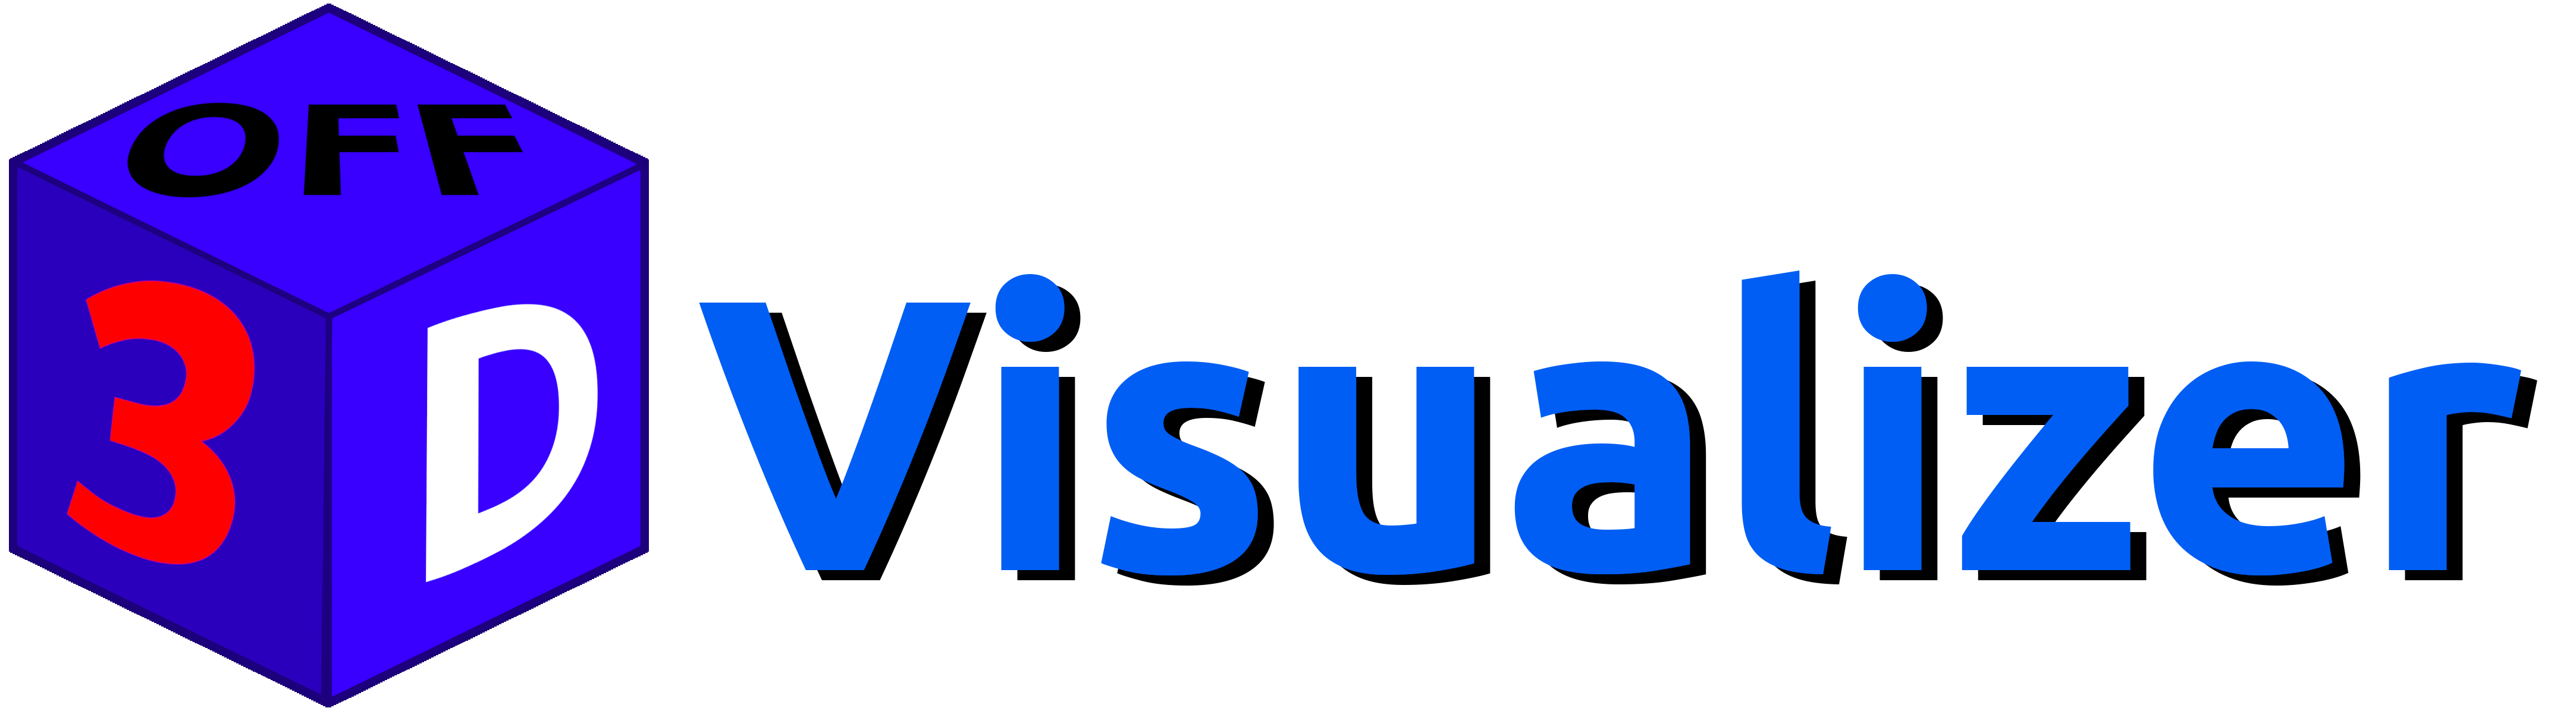
\includegraphics[width=8cm]{logo.png}}

\begin{document}

\maketitle

\tableofcontents
\newpage

\section{Descrição do programa}

Esse programa feito para a disciplina de Computação gráfica, tem como objetivo integrar
C++, Qt e OpenGL, para fazer uma aplicação que seja capaz de abrir arquivos .off (Object File Format),
e ter a capacidade de manipulá-los. O programa em grande parte consiste na implementação do artigo 
\emph{"Interactive Graphics Applications with OpenGL Shading Language and Qt"}, com apenas algumas 
melhoras a sua interface, e a adição a uma funcionalidade de melhoria, que é a leitura de malhas
mistas.

\section{Organização do código}

\section{Detalhando módelos matemáticos}

\end{document}
